%& -shell-escape
\title{Linear Regression}
\author{Ahnaf An Nafee}
\date{March 2021}
\documentclass[12pt]{article}
\usepackage[margin=0.7in]{geometry}
\usepackage{graphicx}
\usepackage{float}
\usepackage{amsmath}
\usepackage{multicol}
\usepackage{comment}
\usepackage{listings}
\usepackage{xcolor}
\usepackage{multirow}

\graphicspath{ {./images/} }

\definecolor{codegreen}{rgb}{0,0.6,0}
\definecolor{codegray}{rgb}{0.5,0.5,0.5}
\definecolor{codepurple}{rgb}{0.58,0,0.82}
\definecolor{backcolour}{rgb}{0.95,0.95,0.92}

\lstdefinestyle{mystyle}{
	backgroundcolor=\color{white},   
	commentstyle=\color{codegreen},
	keywordstyle=\color{magenta},
	numberstyle=\tiny\color{codegray},
	stringstyle=\color{codepurple},
	basicstyle=\ttfamily\footnotesize,
	breakatwhitespace=false,         
	breaklines=true,                 
	captionpos=b,                    
	keepspaces=true,                 
	numbers=left,                    
	numbersep=5pt,                  
	showspaces=false,                
	showstringspaces=false,
	showtabs=false,                  
	tabsize=2
}

\lstset{style=mystyle}


\begin{document}
	
	\maketitle
	
	\section{Theory}
	
	\begin{enumerate}
		\item Target Function:
		
		
		\begin{enumerate}
			
			\item Sample Entropy:\\
			

				$Total = 21$\\ 
				$Positive Count = 12$\\  
				$Negative Count = 9$   \\\\
				
				\begin{equation}
					\begin{split}
						H(Y) = -(\frac{12}{21} \cdot log_2 (\frac{12}{21}) + \frac{9}{21} \cdot log_2 (\frac{9}{21}))
					\end{split}
				\end{equation}
				
				$H(Y) = 0.985228$\\

			
			\item Weighed Average Entropy:\\
			
			\begin{tabular}{ c c}
				$p_0 = 5$ & $n_0 = 8$\\ 
				$p_1 = 7$ & $n_1 = 1$ 
			\end{tabular}
			
			
			\begin{equation}
				\begin{split}
					E(H(1)) = \frac {5+8}{21} \times (\frac{-5}{13} \cdot log_2 \frac{5}{13} + \frac{-8}{13} \cdot log_2 \frac{8}{13}) +\\
					\frac {7+1}{21} \times (\frac{-7}{8} \cdot log_2 \frac{7}{8} + \frac{-1}{8} \cdot log_2 \frac{1}{8})
				\end{split}
			\end{equation}
			
			\begin{equation}
				\begin{split}
					E(H(1)) = 0.802123
				\end{split}
			\end{equation}
		
		
		\begin{tabular}{ c c}
			$p_0 = 5$ & $n_0 = 6$\\ 
			$p_1 = 7$ & $n_1 = 3$ 
		\end{tabular}
		
		
		\begin{equation}
			\begin{split}
				E(H(2)) = \frac {5+6}{21} \times (\frac{-5}{11} \cdot log_2 \frac{5}{11} + \frac{-6}{11} \cdot log_2 \frac{6}{11}) +\\
				\frac {7+3}{21} \times (\frac{-7}{10} \cdot log_2 \frac{7}{10} + \frac{-3}{10} \cdot log_2 \frac{3}{10})
			\end{split}
		\end{equation}
		
		\begin{equation}
			\begin{split}
				E(H(2)) = 0.940344
			\end{split}
		\end{equation}
			
			
			
			\item Decision Tree:\\
			
			\begin{equation}
				\begin{split}
					IG(X_1) = 0.985228 - 0.802123 = 0.183107
				\end{split}
			\end{equation}
		
			\begin{equation}
				\begin{split}
					IG(X_2) = 0.985228 - 0.940344 = 0.044885
				\end{split}
			\end{equation}
			
				\begin{center}
					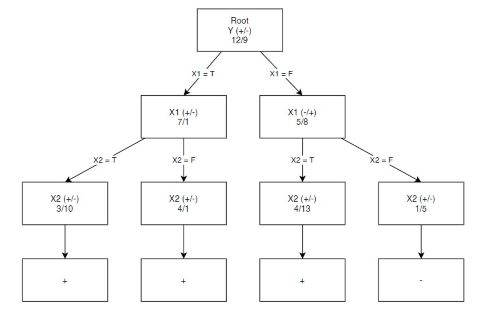
\includegraphics{d_tree_01}
				\end{center}
			
			
		\end{enumerate}
		
		\begin{comment}
		\newpage
		\end{comment}
		
		
		\item Essay Data:\\
		
		\begin{enumerate}
			
			\item Class Priors:\\
			
			\begin{equation}
				\begin{split}
					P(\textit{A = Yes}) = 3/5 = 0.6
				\end{split}
			\end{equation}
		
			\begin{equation}
				\begin{split}
					P(\textit{A = No}) = 2/5 = 0.4
				\end{split}
			\end{equation}
			
			
			
			\item Parameters of the Gaussians:\\
			
			
			
			\item Determine:\\
			
			
		\end{enumerate}
		
		
	\end{enumerate}
	
	\newpage
	
	\section{Naive Bayes Classifier}
	
	\begin{enumerate}
		
		\item Classification Statistics:\\
		
		Precision: $94.54545454545455\%$ \\
		Recall: $69.84126984126983\%$ \\
		F-measure: $80.33707865168539\%$ \\
		Accuracy: $81.7351598173516\%$ \\

		
	\end{enumerate}
	
	
	
	\section{Logistic Regression}
	
	\begin{enumerate}
		
		\item Classification Statistics:\\
		
		Precision: $37.37864077669903\%$ \\
		Recall: $77.77777777777779\%$ \\
		F-measure: $50.49180327868853\%$ \\
		Accuracy: $70.45009784735812\%$ \\
		
		
	\end{enumerate}
	
\end{document}
